\documentclass{book}
\usepackage{xeCJK}
\usepackage{ctexcap}
\usepackage{bm}
\usepackage{amsmath,amssymb,amsfonts}
\usepackage{float}

\begin{document}
\title{电机学与拖动基础}
\chapter{电路}


\chapter{磁路}
\section{基本电磁现象及有关定律}
各种电机都是靠电与磁的相互作用、相互转换而完成能量转换的,所以除电路知识外,电磁基本定律也是分析电机的重要理论基础。

回顾一下,麦克斯韦电磁场理论的基本思想是:\uline{相对时间变化的磁场会产生感生电场,而相对时间变化的电场会产生磁场}。根据这一思想,如果空间某一区域内,有变化的电场(如电荷做加速运动),那么临近区域内就会产生变化的磁场。这个变化的磁场又会在较远处产生变化的感生电场。这样产生出来的电场也是随着时间变化的,它必然要产生新的磁场。这样,在充满变化的电场空间,同时也充满变化的磁场,二者相互联系、相互转化。

\subsection{稳恒磁场}
在运动电荷周围,除了存在电场以外,还存在另外一种性质的场——磁场。

将一个速度为$v$,电荷量为$q$的运动点电荷引入磁场,测量通过磁场中任意给定点$P$的运动点电荷所受的磁力。试验结果归纳如下。
\par (1)\uline{当点电荷沿磁场方向运动时,它不受磁场力作用},$F=0$.

\par (2)\uline{当点电荷垂直于磁场方向运动时,它所受的磁场力最大},用$F_{\max}$表示。这个力的方向垂直于磁场方向与点电荷运动方向所组成的平面,

注意:表征垂直纸面的方向用$\odot$(弓箭迎面而来),$\otimes$(弓箭远离而去,留下个尾巴)。

对磁场中某一点来说,$\frac{F_{\max}}{\left|q\right|v}$是一个与$\left|q\right|v$的大小都无关的恒量,这恒量仅与磁场在该点的性质有关。特别注意:$\frac{F_{\max}}{\left|q\right|v}$只反映$\bm{B}$的大小,并不反映$B$的方向。据此,如图\ref{fig:ap force}所示,可以推导出电流元在磁场中受的安培力为
\[d\bm{F}=Id\bm{l}\times \bm{B}\]
\begin{figure}[H]
	\centering
	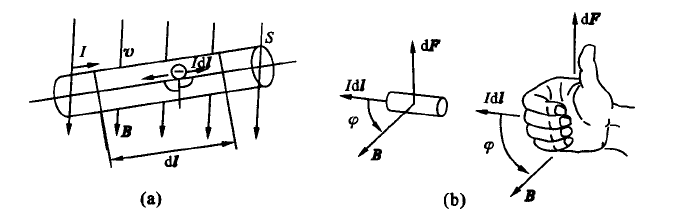
\includegraphics[width=25pc]{apeiforce}
	\caption{安培力}
	\label{fig:ap force}
\end{figure}

\subsubsection{毕奥-萨伐尔定律}

电流元的概念,$Idl$为电流元,它是矢量,其单位为$A \cdot m$(即安$\cdot$米)。

综上所述,可设想:如图\ref{fig:biao}所示,电流元$Idl$在离它距离为$r$的空间某点$P$引起的磁场强度$dB$的大小,与电流元的大小$Idl$成正比,与电流元$Idl$到$P$的距离为$r$的二次方成反比。
$d\bm{B}$的大小为:
\begin{equation}
d\bm{B}=\frac{\mu_{0}Idl\sin\alpha}{4\pi r^2}
\end{equation}
式中:$r$是从电流元所在点到点$P$的距离(相应的矢径为$r$),$\mu_0=4\pi\times 10^{-7}$$T\cdot m\cdot A^{-1}$, $\mu_{0}$称为真空磁导率,$\alpha$为$Id\bm{l}$与$\bm{r}$之间的小于$180^{\circ}$的夹角,$dB$的方向垂直于$Idl$与$r$组成的平面,指向为由$Idl$经$\alpha$角转向$r$时右螺旋前进的方向。
若用矢量式表示,则有
\begin{equation}
d\bm{B}=\frac{\mu_{0}Id\bm{l}\times \bm{r}_0}{4\pi r^2}
\end{equation}
在电机中都是以线圈通电来建立磁场的,电流的大小和方向决定着它所产生磁场的强弱和方向。
\begin{figure}[H]
	\centering
	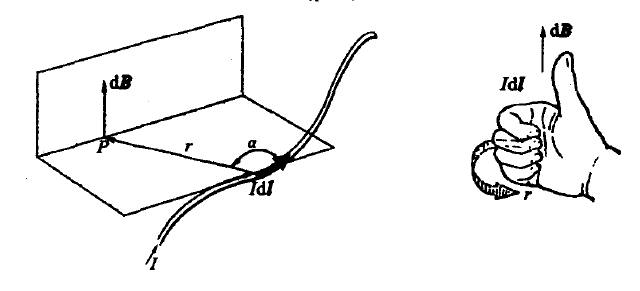
\includegraphics[width=25pc]{biao}
	\caption{电流元所产生的磁感强度}
	\label{fig:biao}
\end{figure}

\subsection{磁路的基本定律}
\subsubsection{磁感线}
磁感线,它是为形象描绘磁场在空间分布而人为描绘出的一系列曲线。由于给定磁场中每一点的磁感应强度$\bm{B}$的大小和方向是确定的,因此要作\uline{一系列假想的曲线,使其上每一点的切线方向和该点磁感应强度}$\bm{B}$的方向一致,而曲线的疏密程度则表示各点$\bm{B}$的大小。几种不同形状的载流导线所产生的磁场的磁感应线。

分析各种形状载流导线周围的磁感线,可以看出它们具有如下特性。

(1)由于磁场中某点的磁场方向是确定的,所以磁场中的\uline{磁感线不会相交}。

(2)\uline{磁场中每一根磁感线都是环绕电流的闭合曲线,没有起点,也没有终点}。磁感线的这个特性和静电场中的电场线不同,静电场中的电场线起始于正电荷,终止于负电荷。

(3)\uline{磁感线的环绕方向与电流方向之间的关系},可用图\ref{fig: B line1}表示。

\begin{figure}[H]
	\centering
	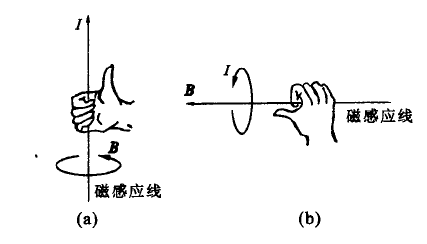
\includegraphics[width=25pc]{magneticfieldline}
	\caption{磁感线环绕方向与电流方向之间的关系}
	\label{fig: B line1}
\end{figure}

\subsubsection{磁路的基尔霍夫第一定律}
由于磁感线是既无起点又无终点的闭合曲线,从一个闭合曲面$S$的某处穿进的磁感线必定从该曲面的另一处穿出。对于闭合曲面来说,规定曲面的外法线方向垂直于曲面向外,因此,从闭合曲面穿出的磁感通量为正,穿入为负。由于磁感线是闭合的,因此对任一闭合曲面来说,穿进闭合曲面的磁感线数目一定等于该闭合曲面的磁感线数目。也就是说,\uline{通过任意闭合曲面的磁通量必等于零},即
\begin{equation}
\mathop{\int\mkern-20.8mu \circlearrowleft}\nolimits_S B\cos\theta dS=\mathop{\int\mkern-20.8mu \circlearrowleft}\nolimits B\cdot dS=0	
\end{equation}

\subsubsection{磁场的基本物理量}
(1) magnetic flux density磁感应强度$B$。它是\textbf{表征某点磁场强弱}的物理量,单位为T(特斯拉)=${Wb}/{{{m}^{2}}}\;$(韦伯/米2)。通常用磁感线来形象的描述磁场,即用磁感线疏密程度表示磁感应强度$B$的大小,磁感线在某点的切线方向就是该点磁感应强度$B$的方向。
对磁感线的密度规定如下:通过磁场中某点处垂直于$\bm{B}$矢量的单位面积上磁感线数目$dN$(磁感线密度)等于该点$\bm{B}$的数值(即$B=\frac{dN}{dS_{\perp}}$)。因此,$B$大的地方,磁感线就密集;$B$小的地方,磁感线就稀疏。

(2) magnetic flux磁通$\Phi $。\uline{它是表征一定范围内磁场总大小的物理量},单位为Wb(韦伯)=$V\cdot s$(伏$\cdot $秒),在匀强磁场中,穿过垂直于磁感应强度$B$的一定面积$S$的磁通量$\phi $,等于$B$与$S$乘积,即:
\begin{equation}
\phi =BS
\label{eq1.1}
\end{equation}	
在非匀强磁场中应用式(\ref{eq1.1})时,磁感应强度$B$应在整个面积$S$内取平均值。

(3)permeability磁导率$\mu $。如果通电环状螺线管中放入一个铁环,则铁环内各点的磁感应强度将会增大很多倍,这说明铁的导磁性能比空气高很多。
物质按它们的磁性质可分为铁磁性质和非铁磁性质两大类。铁磁物质的磁导率远大于真空的磁导率,而所有的非铁磁物质的磁导率都接近于真空的磁导率。磁导率的单位为${H}/{m}\;$(亨利/米)=$\Omega \cdot {s}/{m}\;$(欧$\cdot $秒/米)。

(4) magnetic field intensity磁场强度$H$。为了确定电流与它所产生的磁场之间的数量关系,引入计算量$H={B}/{\mu }\;$,成为磁场强度。

当通入环状螺旋线管的电流$I$一定时,若管中放入铁环,则环内各点的磁感应强度$B$很大;如放入铜环,则环内各点的$B$很小。但在这两种情况下各点的磁场强度$H$不变。可见磁场强度$H$只取决于产生磁场的电流及线圈的物理特征,而与构成磁场的介质的磁性质无关,真正代表磁场各点强弱的磁感应强度$B$与这两方面都有关,即:
\begin{equation}
B=\mu H
\label{eq1.2}
\end{equation}
磁场强度$H$的单位为${A}/{m}\;$(安/米)。
\subsubsection{电机磁路中的概念}
如同把电流流过的路径称为电路一样,磁通所通过的路径称为磁路。不同的是磁通的;路径可以是铁磁物质,也可以是非磁体。图\ref{fig:changjiancilu}所示为常见的磁路。
\begin{figure}[H]
	\centering
	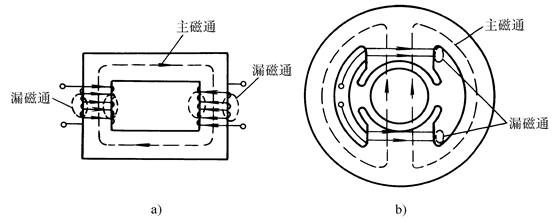
\includegraphics[width=25pc]{changjiancilu}
	\caption{两种常见的磁路 a)变压器磁路 b)两极电流电机磁路}
	\label{fig:changjiancilu}
\end{figure}

在电机和变压器里,常把线圈套装在铁心上,当线圈内通有电流时,在线圈周围的空间(包括铁心内、外)就会形成磁场。由于铁心的导磁性能比空气要好得多,所以绝大部分磁通将在铁心内通过,这部分磁通称为主磁通。围绕载流线圈,在部分铁心和铁心周围的空间,还存在少量分散的磁通,这部分磁通称为漏磁通。主磁通和漏磁通所通过的路径分别构成主磁路和漏磁路,图\ref{fig:changjiancilu}中示意地表示出了这两种磁路。

用以激励磁路中磁通的再留线圈称为励磁线圈,励磁线圈中的电流称为励磁电流。若励磁电流为直流,磁路中的磁通是恒定的,不随时间变化而变化,这种磁路称为直流磁路;直流电机的磁路就属于这一类;若励磁电流为交流,磁路中的磁通是随时间变化而变化的,这种磁路称为交流磁路;交流铁心线圈、变压器、感应电机的磁路都属于这一类。
\subsubsection{磁路的基尔霍夫第二定律}
在磁场中沿任意闭合曲线$L$作磁场强度矢量的线积分,其值等于该闭合曲线所包围的电流的代数和,即
\begin{equation}
\oint_{L}{\vec{H}\cdot d\vec{L}=\sum{I}}
\label{eq1.3}
\end{equation}

在$\sum{I}$中,与积分方向符合右手螺旋关系的电流取正号,反之取负号。例如在图\ref{fig:kvlmag}中,有:
\[\sum{I}={{I}_{1}}+{{I}_{2}}-{{I}_{3}}\]
\begin{figure}[H]
	\centering
	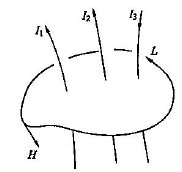
\includegraphics[width=25pc]{kvlmag}
	\caption{磁路的基尔霍夫第二定律}
	\label{fig:kvlmag}
\end{figure}
磁路的基尔霍夫第二定律只说明了$\bm{B}$矢量的环流$\oint_l\bm{B}\cdot d\bm{l}$的值与闭合路径所环绕的电流$\sum_{i}I_i$有关,并非说磁场强度$\bm{B}$只与所围绕的电流有关。这是因为磁场中任一点的磁感应强度总是由激发这磁场的电流所决定的,不管这些电流是否被所取的闭合线所围绕,它们对磁场中任一点的磁场强度$\bm{B}$都是有贡献的。
\subsubsection{磁路欧姆定律}
在电机中,为了能利用较小的电流产生较强的磁场,通常采用铁磁材料制成一定形状的铁心。有了铁心,不仅能使磁场显著增强,而且能使绝大部分的磁通按照设计者所要求的流通路径闭合,构成电机的主磁路。

图\ref{fig:simplemag}所示为一简单磁路,铁心长度为$l$,截图为$S$,线圈匝数为$N$,通入电流为$I$。根据磁路的基尔霍夫第二定律可得
\[Hl=IN\]
\begin{figure}[H]
	\centering
	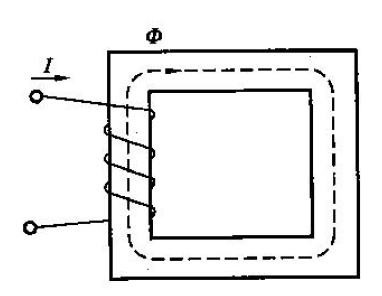
\includegraphics[width=25pc]{simplemag}
	\caption{简单磁路}
	\label{fig:simplemag}
\end{figure}


设铁心的磁导率为$\mu $,则$H={B}/{\mu }\;$,而$B={\phi }/{S}\;$,所以
\[\frac{\phi l}{\mu S}=IN\]
\begin{equation}
\phi =\frac{IN}{\frac{l}{\mu S}}=\frac{F}{{{R}_{m}}}
\label{eq1.4}
\end{equation}

式中$F$——产生磁通$\phi $的原动力,称为magnetomotive force磁动势,$F=IN$;

${{R}_{m}}$——磁路的磁阻,${{R}_{m}}=\frac{l}{\mu S}$。

式(\ref{eq1.4})称为磁路欧姆定律。



实际电机、电器的磁路,根据材料和截面的不同常分为若干段,这时应用磁路的基尔霍夫定律得

\[{{H}_{1}}{{l}_{1}}+{{H}_{2}}{{l}_{2}}+\cdots +{{H}_{n}}{{l}_{n}}=IN\]

我们把$H_il_i$称为磁位降。

经推导得

\begin{equation}
\Phi =\frac{IN}{\frac{{{l}_{1}}}{{{\mu }_{1}}{{S}_{1}}}+\frac{{{l}_{2}}}{{{\mu }_{2}}{{S}_{2}}}+\cdots +\frac{{{l}_{n}}}{{{\mu }_{n}}{{S}_{n}}}}=\frac{F}{\sum{{{R}_{m}}}}
\label{eq1.5}
\end{equation}	

式中,$\sum{{{R}_{m}}}$——各段磁路磁阻之和,也就是整个闭合磁路的总磁阻。

\subsubsection{电感计算}
\begin{figure}[H]
	\centering
	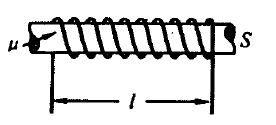
\includegraphics[width=25pc]{luoxianguan}
	\caption{长直螺线管}
	\label{fig:luoxianguan}
\end{figure}
真空中,一无限长螺线管长$l=50 \text{cm}$,截面积$S=10 \text{cm}^2$,单层密绕$N=3000$匝,试求其电感系数。
\par 由于此螺线管的长度远大于它的直径,在计算时可近似看作是无限长的。当螺线管通有电流$I$时,根据毕奥-萨伐尔定律可计算管内匀强磁场的磁感应强度为:
\begin{equation}
	B=\mu_{0}nI
\end{equation}
式中:$n=\frac{N}{l}$为单位长度的匝数。通过每一匝的磁通量都等于
\begin{equation}
	\phi=BS=\mu_{0}nIS
\end{equation}
通过整个螺线管的磁链(Flux Linkage)为:
\begin{equation}
	\psi=N\phi=\mu_0 n N I S=\mu_0\frac{N^2}{l}IS
\end{equation}
根据电感系数的定义:
\begin{equation}
	L=\frac{\psi}{I}
\end{equation}

磁阻${{R}_{m}}=\frac{l}{{{\mu }_{r}}{{\mu }_{0}}S}$,
电感系数:$L=\frac{{{N}^{2}}}{{{R}_{m}}}$,
在交流稳态电路分析时,对应电抗的计算为:$\omega L$,由此可得到重要的定性规律:电抗大,电感大,磁阻小,磁导率大。

\subsubsection{气隙的边缘效应}
\uline{磁路中与空气隙时,气隙边缘的磁感应线将由向外扩张的趋势,称为边缘效应},如图\ref{fig:qixi bianyuan}。工程上一般认为,当气隙较小时,可用下面两式计算气隙的有效面积:
当截面为矩形($a\times b$)截面时,气隙有效面积$S_0=\left(a+\delta_0\right)\left(b+\delta_0\right)$。当截面为圆形($\pi r^2$)截面时,气隙有效面积$S_0=\pi\left(r+\delta_0\right)^2$。
%qixibianyuan
\begin{figure}[H]
	\centering
	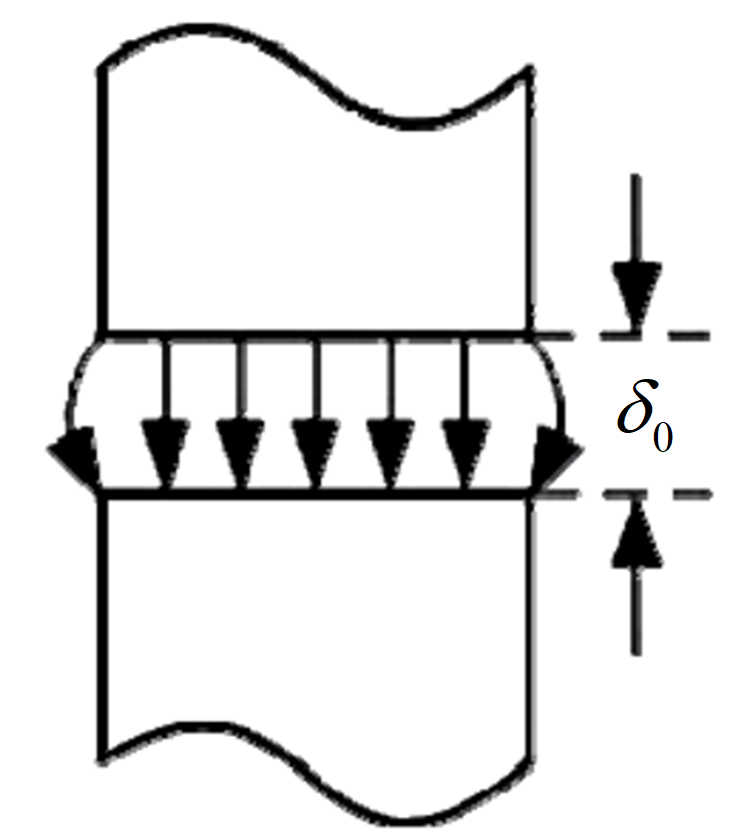
\includegraphics[width=25pc]{qixibianyuan}
	\caption{气隙的边缘效应}
	\label{fig:qixi bianyuan}
\end{figure}

\section{电磁感应}
前面研究了静电场和稳恒磁场的基本规律,我们知道,静电场和稳恒磁场是各自独立、互不相关的。但是,激发静电场和稳恒磁场的源————电荷和电流却是相互关联的,这就可以联想到电场和磁场之间也一定存在着相互联系、相互制约的关系。
\par 历史上进行了许多实验研究,终于发现了电磁感应现象:即当穿过闭合导体回路中的磁通量发生变化时,回路中即出现了电流。这一重大发现,不仅阐明了变化磁场能够激发电流这一关系,还进一步揭示了电与磁的内在联系,促进了电磁理论的发展。



英国科学家法拉第于1821年做了最早的电动机实验模型的尝试,并与1831年发现了电磁感应定律——当磁场的磁力线发生变化时,在其周围的导线中就会感应产生电流,其数学表达式为:
\begin{equation}
e=-\frac{d\psi }{dt}
\label{eq1.6}
\end{equation}

式中,$\psi $——磁链,当其通过具有$N$匝的线圈时,有$\psi =N\phi $,$\phi $为单匝线圈中通过的磁通量。式(\ref{eq1.6})可写为
\begin{equation}
e=-\frac{d\psi }{dt}=-N\frac{d\phi }{dt}
\label{eq1.7}
\end{equation}

\subsection{楞茨定律}
1833年,楞次在总结大量实验结果的基础上,提出了一个判定电磁感应中感应电流方向的法则,称为楞次定律。楞次定律说:闭合回路中的感应电流的方向,是要使感应电流在回路所围面积上产生的磁通量,去抵消或反抗引起感应电流的磁通量的变化。楞次定律表明,\uline{电磁感应的结果反抗电磁感应的原因}。这里的结果是指感应电流所产生的磁通量,原因是指引起电磁感应的磁通量的变化。
考虑如图\ref{fig: lengci}所示的那样一个实验,一块条形磁铁穿过一个闭合线圈的过程。图(a)是磁铁向左运动靠近线圈的情况。这时线圈中的磁场$\bm{B}$向左且在增强,故磁通量$\phi$在增加,按楞次定律,感应电流$I'$的磁通量$\phi'$应反抗$\phi$的增加,即感应电流在线圈中的磁场$\bm{B}'$应与$\bm{B}$方向相反即向右,再由右手螺旋法则就可以确定感应电流$I'$的方向应如图\ref{fig: lengci}(a)所示。图(b)是磁铁已穿过线圈继续向左运动的情况。这时磁场$\bm{B}$仍向左但在减小,故磁通量$\bm{B}$在减小。按楞次定律,感应电流的磁通量$\phi'$应反抗$\phi$的减小,即感应电流的磁场$B'$应与$B$方向相同即向左,故感应电流的方向应与(a)中相反。
\begin{figure}[H]
	\centering
	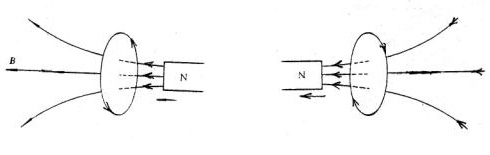
\includegraphics[width=25pc]{lengci}
	\caption{感应电流的方向}
	\label{fig: lengci}
\end{figure}
借助上述实验可以说明楞次定律的物理意义。在实验中闭合线圈里有感生电流产生,于是线圈中应有能量释放出来,如发出焦耳热。应该考虑一下,这些能量究竟是从哪儿来的?看图(a),电磁感应在闭合线圈上产生的电流会形成一个磁矩,按右手螺旋法则,磁矩向右,即右边是N极。线圈的N极会排斥磁铁的N极,阻止它的相对运动。因而,要进行电磁感应,磁铁就必须要克服斥力而做功,通过做功,磁铁运动的机械能转化为了电能。图(b)中的情况读者可以自己分析,这时线圈的左面是N极,它会通过吸引来反抗相对运动,在这个过程中磁铁也要克服引力做功,把机械能转换为电能。可见电磁感应中释放的能量并不是凭空而来的,而是其它能量如机械能转换而来的。如果楞次定律不是感应电流的磁通量去反抗引起感应电流的磁通量的变化而是支持这种变化,那么上述实验中的一切都会倒过来,那物理学就真会天下大乱了。试想在图(a)中,我们只须给磁铁一点很少的启动能量使之向左运动,如果楞次定律反过来,那么磁铁受到的就将是引力而不是斥力,它就会加速通过线圈,然后继续加速向左运动。在左侧安装一个弹性壁使之反弹向左并继续加速,然后反弹加速……。这样我们就能在磁铁上获得源源不绝的机械能,在线圈上获得无穷无尽的电能,而我们却没有输入任何能量。可见,楞次定律中的反抗的含义就是要强迫外界为电磁感应的进行输入能量,借以提供感应中的能量输出,这显然是在维护能量守恒定律这个自然界的普遍法则在电磁感应中的地位。所以我们说,楞次定律是能量守恒定律在电磁感应中的具体表现。这不仅是在上述实验中是如此,实际上,电磁感应的所有实验都验证了能量守恒定律。
基于楞茨定律,可判断感应电动势的方向:
\begin{figure}[H]
	\centering
	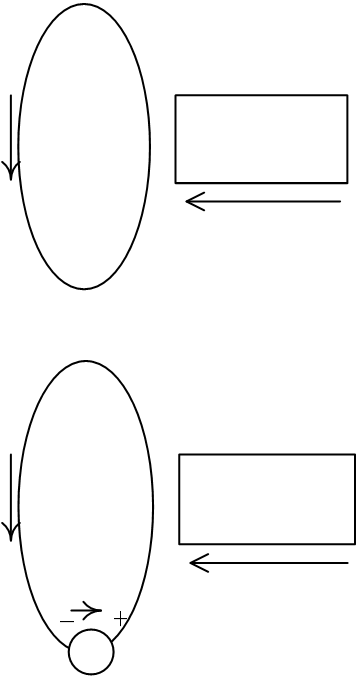
\includegraphics[width=25pc,height=32pc]{lenz}
	\caption{楞次定律感应电动势的方向}
	\label{fig:lenz}
\end{figure}
\subsection{磁通变化感生电动势}
当穿过线圈的磁通$\Phi $发生变化时,在线圈中将产生电动势$e$,其大小与磁通变化率成正比,还与线圈的匝数$N$成正比;$e$的方向总是企图产生一个阻碍原磁通变化的电流。

在图中,$\Phi $增大时,$e$的方向由b到a;$\Phi $减少时,$e$的方向由a到b。为了便于分析计算,必须规定$e$的正方向。按照电工惯例,$\Phi $与$e$两者的正方向应符合右手螺旋定则,所以在中$e$的正方向应是从$a$到$b$。可见,当$\Phi $减少$\left( \frac{\text{d}\Phi }{\text{d}t}<0 \right)$时,$e$的真实方向与其正方向一致(即$e>0$);而当$\Phi $增大$\left( \frac{\text{d}\Phi }{\text{d}t}>0 \right)$时,$e$的真实方向与其正方向相反$\left( e<0 \right)$。

\uline{应用式判断感应电动势}$e$的方向时,必须先按右手螺旋定则规定$\Phi $与$e$的正方向,然后根据$\frac{\text{d}\Phi }{\text{d}t}$的正负,由上式确定$e$的符号。
\subsection{导体切割磁通感生电动势}
直导体在磁场中做切割磁力线的运动时,在导体中将产生感应电动势$e$。如果磁场方向、导体放置方向和导体运动方向三者相互垂直,则感应电动势$e$的大小为:
\begin{equation}
e=BLv
\label{eq1.8}	
\end{equation}
式中$B$——磁感应强度,T;

$L$——导体有效长度,m;

$v$——运动速度,m/s;

$e$——感应电动势,V。

感应电动势$e$的方向\uline{可用右手定则来判定},手心迎着磁场方向,大拇指指向导体运动方向,则其他四指指向方向为$e$的方向,也是电流方向。\uline{也可以用洛伦兹力判断正电荷流向}。
\subsection{电磁力}
通电导体在磁场中受到力的作用,这种力称为电磁力,当电流方向与磁场方向相互垂直时,电磁力的大小为:
\[F=BLI\]

电磁力$F$的方向\uline{用左手定则来判定},手心迎着磁场方向,四指代表电流方向,则大拇指所指方向为电磁力方向。


\section{铁磁物质的基本磁特性}
作为电机重要结构部件的铁心都是用\uline{铁磁物质}制成的,铁磁物质还包括\uline{铁、钴、镍}以及它们的合金。
铁磁ferro-magnetic
\subsection{铁磁物质的主要性质}
\subsubsection{高导磁性}
如果在图\ref{fig_1.1}的环状螺旋线管中放入一个铁磁物质制成的圆环,管中各点的磁感应强度就可能增强数百倍,这说明铁磁物质的磁导率远远大于非铁磁物质。铁磁物质具有高导磁性,是因为在铁磁物质内部存在着大量的被称作磁畴的微小磁体。当铁磁物体未处于磁场中时,其内部的磁畴呈杂乱无章的排列状态,见图\ref{fig_1.2} (a),对外不显现磁性。当将铁磁物体放入磁场时,在外磁场作用下,磁畴将按外磁场的方向取向排列,如图\ref{fig_1.2} (b)所示,\uline{形成一个比原外磁场大许多倍的附加磁场,这个过程称为铁磁物质的磁化。}

可见,铁磁物质具有高导磁性的实质是它能被磁化。人们利用它的这种性质构成各种各样所需的此路。

\begin{figure}[H]
	\centering
	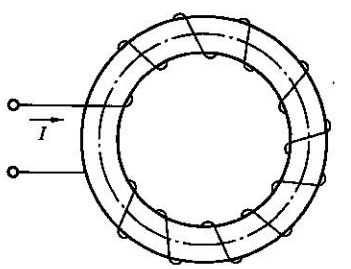
\includegraphics[width=0.80\textwidth]{1-1.png}
	\caption{环状螺线管}
	\label{fig_1.1}
\end{figure}

\begin{figure}[H]
	\centering
	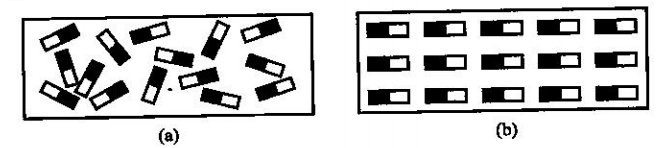
\includegraphics[width=0.80\textwidth]{1-2.png}
	\caption{磁畴}
	\label{fig_1.2}
\end{figure}

\subsubsection{磁饱和}
对于上述带有铁心的环状螺线管,当通入其中的电流$I$从零逐渐增大时,铁心中各点的磁场强度$H$和磁感性强度$B$也都将随之增大,然而$H$和$B$的增长规律却不完全相同。图\ref{fig_1.3}所示为$B=f\left( H \right)$曲线,称作铁磁物质的磁化曲线。在曲线中oa段上,当$H$值随电流$I$成正比增大时,$B$值增大较快,且大致和$H$成正比。在ab段上,$B$值增长逐渐缓慢,这是因为大部分磁畴已按$H$的方向排列,可以转向的磁畴越来越少。在b点以后,磁化过程基本结束,$B$值增加更加缓慢,因为这时只有螺线管中电流起增强磁场的作用,$B$值增加的速度与无铁心时一样。由于磁化趋于结束和完全结束而使铁心中$B$值增长变缓的现象称为磁饱和。磁饱和使铁心的导磁系数$\mu =\frac{B}{H}$变小,磁阻${{R}_{m}}=\frac{L}{\mu S}$变大。磁饱和程度越高,$\mu $值越小,${{R}_{m}}$值越大。可见磁饱和造成了磁路的非线性(磁通和磁动势不成正比),给磁路的分析、计算增加了难度。\uline{可以根据这一特性,画出电感随电流的变化曲线}。
\begin{figure}[H]
	\centering
	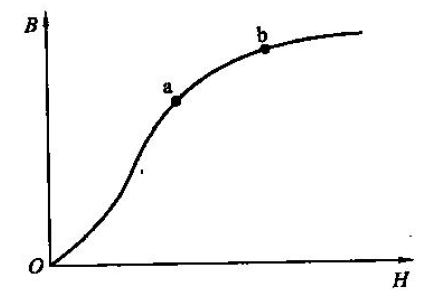
\includegraphics[width=0.80\textwidth]{bhfig.png}
	\caption{$B=f\left( H \right)$曲线}
	\label{fig_1.3}
\end{figure}

\subsubsection{磁滞}
当螺线管通入交变电流时,铁心中的磁场强度$H$和磁感应强度$B$也将随之交变。这时铁心中的磁畴也将不断地翻转,以改变方向。\uline{由于磁畴之间的互相摩擦,使得它们取向排列的步调跟不上外磁场的变化步调},即$B$的变化滞后于$H$的变化,这种现象称为磁滞。$B$随$H$的变化关系曲线称为磁滞回线,如图\ref{fig_1.4}所示。

在图\ref{fig_1.4}中,当$H$由$+{{H}_{m}}$减少为零时,$B$仍将保持一定数值,称为剩磁感应强度。如果回线横向宽度较宽,铁磁物质的磁滞性越强,剩磁越大,称为硬磁材料,工程上多用此材料制成永久磁铁。如果回线横向宽度较窄(回线所围成的面积较小),磁滞性较弱,则称为软磁材料,电机、变压器等铁心是用软磁材料制成的。磁滞现象将影响通过电流调节磁场强弱的效果,同时磁滞还将在铁心中产生能量损耗。
\begin{figure}[H]
	\centering
	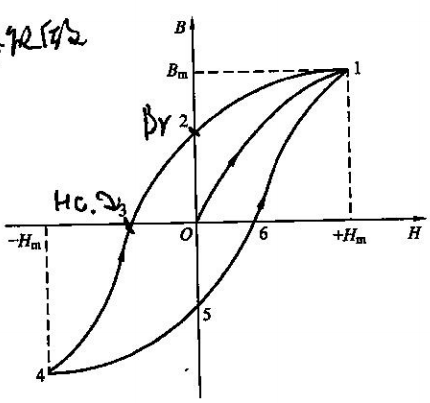
\includegraphics[width=0.80\textwidth]{1-4.png}
	\caption{铁磁材料的磁滞回线}
	\label{fig_1.4}
\end{figure}

\subsection{铁心损耗}
\subsubsection{磁滞损耗}
\uline{当通过铁心的磁通交变时,由于不断翻转的磁畴之间的相互摩擦而使铁心发热,由此引起的能量损失称为磁滞损耗}。
\subsubsection{涡流损耗}
当通过铁心的磁通交变时,在铁心的表面上将产生感应电动势,并形成漩涡状的电流,称为涡流[见图\ref{fig_1.5}]。涡流在铁心中流动造成能量损失,使铁心发热,称为涡流损耗,如图\ref{fig_1.5}(a)所示,为了减少涡流损耗,常通过交变磁通的铁心不用整块的铁,而是\uline{用相互绝缘的硅钢片叠压制成},如图\ref{fig_1.5}(b)所示。硅钢片的厚度一般为0.35\textasciitilde0.5mm,这样涡流就无法顺畅地通过整个铁心横截面闭合,而只能在每片内构成局部涡流。由于穿过每片的磁通很小,再加上涡流的路径很窄,电阻很大,从而使涡流大为削弱。钢中加入硅,使电阻率变大,可进一步减少涡流和涡流损耗。
\begin{figure}[H]
	\centering
	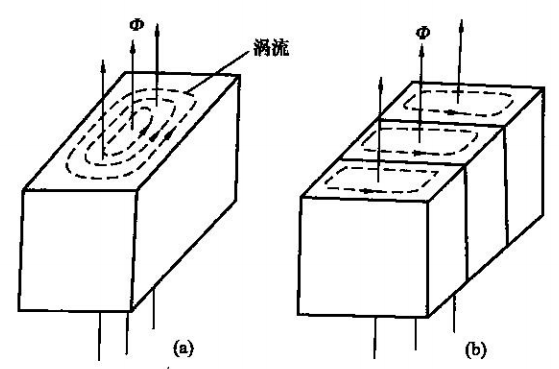
\includegraphics[width=0.80\textwidth]{1-5.png}
	\caption{(a)涡流损耗;(b)用硅钢片减少涡流损耗}
	\label{fig_1.5}
\end{figure}

\uline{磁滞损耗和涡流损耗合在一起,称为铁心损耗},它的大小取决于铁心中交变磁感应强度的最大值${{B}_{m}}$和磁通交变的频率$f$。工程上采用下列经验公式计算包括磁滞和涡流损耗在内的铁心损耗,即
\begin{equation}
{{p}_{Fe}}={{P}_{1/50}}{{\left( \frac{f}{50} \right)}^{\beta }}B_{m}^{2}G
\label{eq9}
\end{equation}	

式中  $\beta $——指数,在1.3\textasciitilde1.6之间取值;

${{P}_{1/50}}$——与材料有关的系数,同时又取决于所用单位;

$G$——铁心的体积。

\subsection{铜损耗}
\uline{铜损是电流通过绕组时,在绕组的电阻上所消耗的功率,铜损又叫可变损耗}。

\section{直流磁路的计算}
磁路计算有两种类型,一类是给定磁通量,计算所需的励磁磁动势,称为磁路计算的正问题;另一类是给定励磁磁动势,求磁路内的磁通量,称为磁路计算逆问题。电机的磁路计算通常属于第一类。

对于磁路计算的正问题,步骤如下:

1)	将磁路按材料性质和不同截面尺寸分段;

2)	计算各段磁路的有效截面积${{A}_{k}}$和平均长度${{l}_{k}}$ ;

3)	计算各段磁路的平均磁通密度${{B}_{k}}$,${{B}_{k}}={{{\Phi }_{k}}}/{{{A}_{k}}}\;$;

4)	根据${{B}_{k}}$求出对应的磁场强度${{H}_{k}}$,对铁磁材料,${{H}_{k}}$可从基本磁化曲线上查出;对于空气隙,可直接用${{H}_{\delta }}={{{B}_{\delta }}}/{{{\mu }_{0}}}\;$算出。

5)	计算各段磁位降${{H}_{k}}{{l}_{k}}$,最后求出$~F=\sum{{{H}_{k}}{{l}_{k}}}$。

对于逆问题,由于磁路是非线性的,常用试探法去求解。

\subsection{简单串联磁路}
简单串联磁路就是不及漏磁影响,仅有一个磁回路的无分支磁路,如图\ref{fig_chuanliancilu}所示。此时通过整个磁路的磁通量相同,但由于各段磁路的截面积不同或材料不同,各段的磁通密度也不一定相同。这种磁路虽然简单,却是磁路计算的基础。下面举例说明。
\begin{figure}[H]
	\centering
	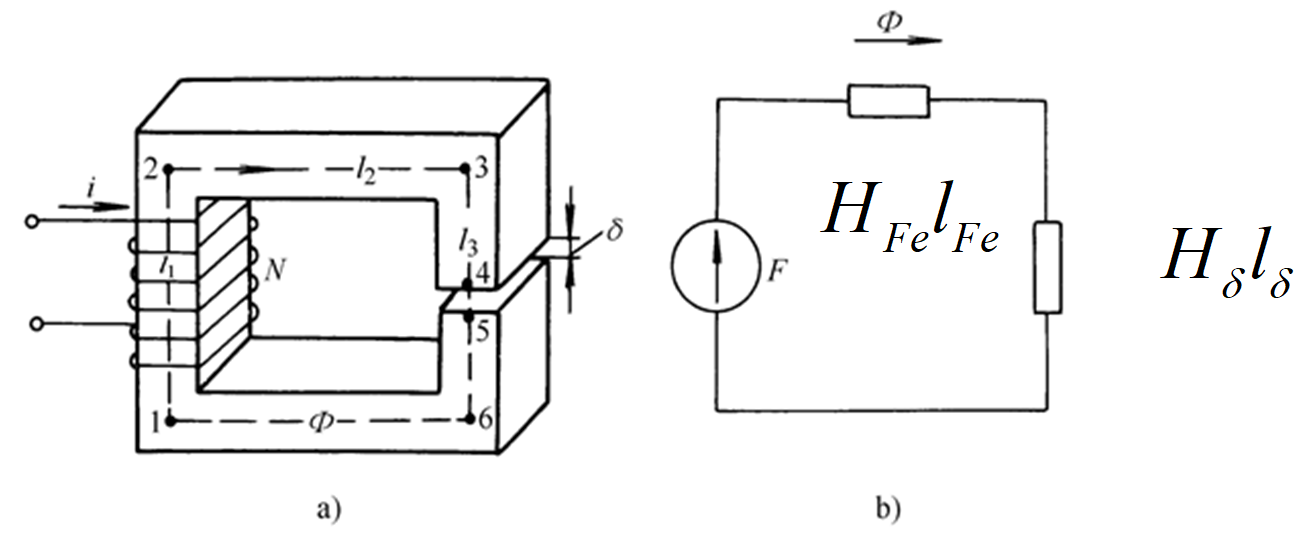
\includegraphics[width=0.80\textwidth]{chuanliancilu.png}
	\caption{简单串联磁路 a)串联磁路 b)模拟电路图}
	\label{fig_chuanliancilu}
\end{figure}

\begin{figure}[H]
	\centering
	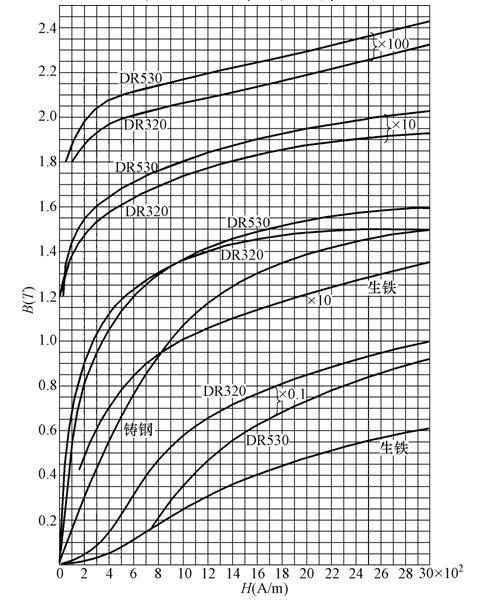
\includegraphics[width=0.80\textwidth]{cihuaquxian.png}
	\caption{电机中常用铁磁材料的基本磁化曲线}
	\label{fig_cihuaquxian}
\end{figure}

【例题】 磁路铁心材料由铸钢和空气隙构成,铁心截面积${{A}_{Fe}}=3\times 3\times {{10}^{-4}}{{\text{m}}^{2}}$,磁路的平均长度${{l}_{Fe}}=0.3\text{m}$,气隙长度$\delta =5\times {{10}^{-4}}\text{m}$,见图1-13。求该磁路获得磁通量$\Phi =0.0009\text{Wb}$时所需要的励磁磁动势。考虑到气隙磁场的边缘效应,在计算气隙有效面积时,通常再长、宽方向各增加一个$\delta $值。

解:铁心内磁感应强度为
${{B}_{Fe}}=\frac{\Phi }{{{A}_{Fe}}}=\frac{0.0009}{3\times 3\times {{10}^{-4}}}=1\text{T}$

从图\ref{fig_cihuaquxian}中铸钢磁化取现查得,与磁感应强度所应的磁场强度为
\[{{H}_{Fe}}=9\times {{10}^{2}}\text{A}/m\]

则铁心段的磁位降 \[{{H}_{Fe}}{{l}_{Fe}}=9\times {{10}^{2}}\times 0.3\text{A}=270\text{A}\]

空气隙内的磁通密度 \[{{B}_{\delta }}=\frac{\Phi }{{{A}_{\delta }}}=\frac{0.0009}{{{3.05}^{2}}\times {{10}^{-4}}}\text{T}=0.967\text{T}\]

空气内的磁场强度 \[{{H}_{\delta }}=\frac{{{B}_{\delta }}}{{{\mu }_{0}}}=\frac{0.967}{4\pi \times {{10}^{-7}}}\text{A/m}=77\times {{10}^{4}}\text{A/m}\]

空气隙中磁位降 \[{{H}_{\delta }}{{l}_{\delta }}=77\times {{10}^{4}}\times 5\times {{10}^{-4}}\text{A}=385\text{A}\]

总的励磁磁动势 \[F={{H}_{Fe}}{{l}_{Fe}}+{{H}_{\delta }}{{l}_{\delta }}=655\text{A}\]

\subsection{简单并联磁路}
简单并联磁路是指考虑漏磁影响,或磁路有两个以上分支。电机和变压器的磁路大多属于这一类。

【例题】图\ref{fig_bingliandianlu}所示并联磁路,铁心所用材料为DR530硅钢片,铁心柱和铁轭的截面积均为${{A}_{Fe}}=2\times 2\times {{10}^{-4}}{{\text{m}}^{2}}$,磁路铁心段的平均长度${{l}_{Fe}}=5\times \text{ }{{10}^{-2}}m$,气隙长度均为${{\delta }_{1}}={{\delta }_{2}}=2.5\times \text{ }{{10}^{-3}}m$,两个励磁线圈匝数均为${{N}_{1}}={{N}_{2}}=1000$匝。不计漏磁通,试求在气隙内产生${{B}_{\delta }}=1.211\text{T}$的磁感应强度时,所需的励磁电流$i$。
\begin{figure}[H]
	\centering
	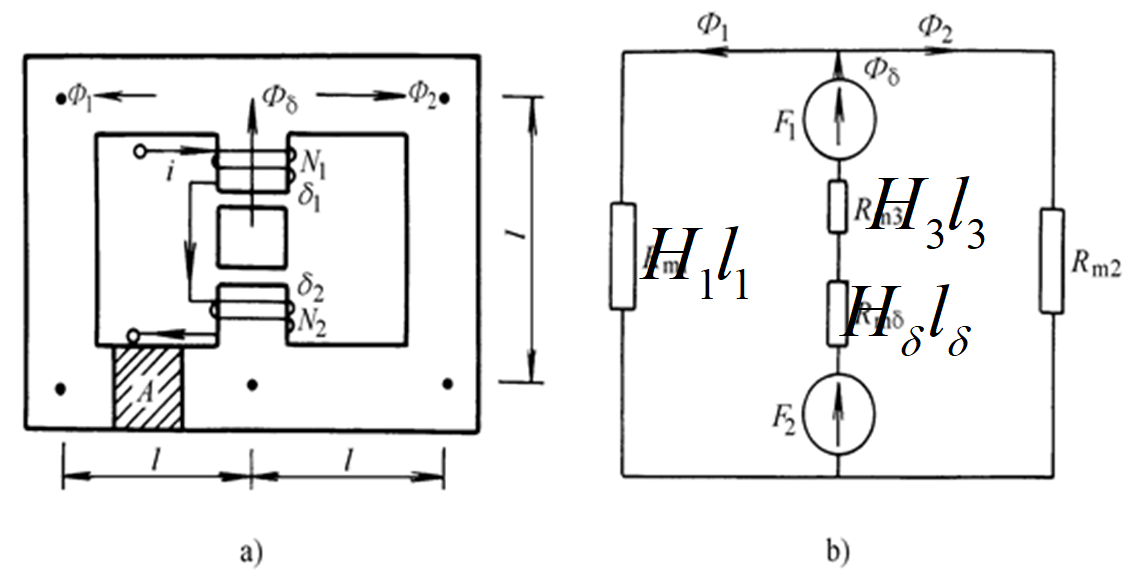
\includegraphics[width=0.80\textwidth]{bingliandianlu.png}
	\caption{简单并联磁路 a)并联磁路 b)模拟电路图}
	\label{fig_bingliandianlu}
\end{figure}

解:由于此路是并联且对称的,故只需计算其中一个磁回路即可。

根据磁路基尔霍夫第一定律,得
\[{{\Phi }_{\delta }}={{\Phi }_{1}}+{{\Phi }_{2}}=2{{\Phi }_{1}}=2{{\Phi }_{2}}\]

根据磁路基尔霍夫第二定律,得
\[\sum{{{H}_{k}}{{l}_{k}}}={{H}_{1}}{{l}_{1}}+{{H}_{3}}{{l}_{3}}+2{{H}_{\delta }}\delta ={{N}_{1}}{{i}_{1}}+{{N}_{2}}{{i}_{2}}\]

由图\ref{fig_bingliandianlu} a)知,中间铁心段的磁路长度
\[{{l}_{3}}=1-2\delta =(5-0.5)\times {{10}^{-}}^{2}\text{m}=4.5\times {{10}^{-}}^{2}\text{m}\]

左、右两边铁心段的磁路长度均为
\[{{l}_{1}}={{l}_{2}}=3l=3\times 5\times {{10}^{-}}^{2}\text{m}=15\times {{10}^{-}}^{2}\text{m}\]

(1)	气隙磁位降
\[2{{H}_{\delta }}\delta =2\frac{{{B}_{\delta }}}{{{\mu }_{0}}}\delta =2\times \frac{1.211}{4\pi \times {{10}^{-7}}}\times 2.5\times {{10}^{-3}}\text{A}=4818\text{A}\]

(2)	中间铁心段的磁位降
\[{{B}_{3}}=\frac{{{\Phi }_{\delta }}}{A}=\frac{1.211\times {{\left( 2+0.25 \right)}^{2}}\times {{10}^{-4}}}{4\times {{10}^{-4}}}\text{T}=1.533\text{T}\]

从图\ref{fig_cihuaquxian}中DR530的磁化曲线查得,与${{B}_{3}}$对应的${{H}_{3}}=19.5\times {{10}^{2}}\text{A/m}$,则中间铁心段的磁位降
\[{{H}_{3}}{{l}_{3}}=19.5\times {{10}^{2}}\times 4.5\times {{10}^{-2}}\text{A=87}\text{.75A}\]

(3)	左、右两边铁心的磁位降磁通密度
\[{{B}_{3}}={{B}_{2}}=\frac{{{{\Phi }_{\delta }}}/{2}\;}{A}=\frac{0.613\times {{{10}^{-3}}}/{2}\;}{4\times {{10}^{-4}}}\text{T}=0.766\text{T}\]

由DR530的磁化曲线查得,${{H}_{1}}={{H}_{2}}=215\text{A/m}$,由此得左、右两边铁心段的磁位降
\[{{H}_{1}}{{l}_{1}}={{H}_{2}}{{l}_{2}}=215\times 15\times {{10}^{-2}}\text{A=32}\text{.25A}\]

(4)	总磁动势和励磁电流为
\[\begin{aligned}
& \sum{Ni}=2{{H}_{\delta }}\delta +{{H}_{3}}{{l}_{3}}+{{H}_{1}}{{l}_{1}}=\left( 4818+87.75+32.25 \right)\text{A=4938A} \\ 
& i=\frac{\sum{Ni}}{N}=\frac{4938}{2000}\text{A}=2.469\text{A} \\ 
\end{aligned}\]

\section{交流磁路的特点}
在铁心线圈中通以直流电流来励磁,分析(直流磁路)要简单些,因为励磁电流是恒定的,在线圈内和铁心中不会产生感应电动势,在一定的电压$U$下,线圈中的电流决定于线圈本身的电阻,功率损耗也只有${{I}^{2}}R$。铁心线圈中通以交流电流时,因为电流是随时间变化的,其电磁关系(电压和电流关系及功率损耗等方面)与直流磁路有所不同。但在每一瞬间仍和直流磁路一样,遵循磁路的基本定率,可以使用相同的基本磁化曲线。磁路计算时,为表明磁路的工作点和饱和情况,磁通量和磁通密度均用交流的瞬时的最大值表示,磁动势和磁场强度则用有效值表示。

交变磁通除了会在铁心中引起损耗之外,还有以下两个效应:

(1)	磁通量随时间变化,必然会在励磁线圈中产生感应电动势$e=-N\frac{d\Phi }{dt}$。

(2)	磁饱和现象会导致励磁电流、磁通和电动势波形的畸变。

\subsection{交流磁路并联}
根据磁路用电路代替的思想,交流磁路并联,对应电路中电感串联。

\subsection{交流磁路串联}
根据磁路用电路代替的思想,交流磁路串联,对应电路中电感并联。
\end{document}
